\documentclass[11pt,twoside,slovak,a4paper]{article}

\usepackage[slovak]{babel}
\usepackage[IL2]{fontenc} % lepšia sadzba písmena Ľ než v T1
\usepackage[utf8]{inputenc}
\usepackage{graphicx}
\usepackage{url} % príkaz \url na formátovanie URL
\usepackage{hyperref} % odkazy v texte budú aktívne (pri niektorých triedach dokumentov spôsobuje posun textu)

\usepackage{cite}

\oddsidemargin=0cm % text na neparnych stranach bude vycentrovany lebo margin = 0
\evensidemargin=0cm
\textwidth=16.5cm % sirka textu na strane

\pagestyle{headings}

\title{Využitie statickej analýzy kódu pri vývoji softwaru}

\author{Lukáš Častven\\[2pt]
	{\small Slovenská technická univerzita v Bratislave}\\
	{\small Fakulta informatiky a informačných technológií}\\
	{\small \texttt{xcastven@stuba.sk}}
	}

\date{\small  5. november 2021}

\begin{document}

\maketitle

\begin{abstract}
	Statická analýza je proces, pri ktorom je počítačový kód zanalyzovaný bez samotného spúšťania kódu.
	Po tejto procedúre, sú programátorovi prezentované nájdené chyby, ich možný spôsob opravy a aj varovania
	o menej závažných nedostatkoch a ich riešenia. Pomocou tejto metódy dokážeme v celom analyzovanom projekte
	zlepšiť kvalitu kódu a udržať konzistentný štýl, ktorý taktiež spĺňa osvedčené postupy pri vývoji softvéru.
	Veľkou výhodou je tiež urýchlenie hľadania chýb a softvérových defektov v porovnaní s manuálnou kontrolou.
	V tomto článku pochopíme, prečo developeri používajú nástroje statickej analýzy, ako ich používajú
	na opravu a zlepšenie kódu a ako ich implementujú do ich pracovného prostredia.
\end{abstract}

\pagestyle{plain}

\section{Úvod}
S rastom komplexity vyvýjaného softvéru, rastie aj jeho minimálna požadovaná kvalita. Chyby a defekty softvéru
dokážu firmám spôsobiť nemalé finančné straty. Preto existujú viaceré metódy ako kvalitu softvérových riešení zlepšiť
a udržať počas vývoja, napríklad podrobné testovanie alebo revízie nového kódu iným developerom. V tomto článku si
bližšie priblížime metódu statickej analýzy, ktorá je používaná na odhalenie chýb a defektov a na udržovanie kvality
kódu na požadovanej úrovni.~\cite{BrittanyJohnson,LisaNguyen}

O statickej analýze samotnej sa dozvieme v časti \ref{principy}, presnejšie, pochopíme čo to je (č.\ref{principy:co}) a
ako funguje (č.\ref{principy:ako}). Ako sa nástroje statickej analýzy používajú v praxi je uvedené v časti
\ref{vyuzitie}, kde zistíme ich benefity (č.\ref{vyuzitie:benefity}) a aj nedostatky (č.\ref{vyuzitie:nedostatky}).
Implementácia v pracovnom prostredí je podrobnejšie vysvetlená v časti \ref{implementacia}, aké formy sa využívajú
(č.\ref{implementacia:formy}) a ako vlastne vyzerá práca za použitia statickej analýzy z pohľadu developera
(č.\ref{implementacia:dev}).

\pagebreak

\section{Princípy statickej analýzy} \label{principy}
\subsection{Čo je statická analýza} \label{principy:co}
Statická analýza je proces, pri ktorom je kód posudzovaný bez spustenia samotného programu a bez vstupu. Preto sa
nazýva statická. Analyzuje sa zdrojový kód a v niektorých prípadoch aj objektový kód\footnote{Väčšinou ide o súbori s
	rozšírením nazvu „.o".}. Po úspešnom ohodnotení kódu, sú developerovi zobrazené nájdené chyby a defekty. Taktiež sú
poskytnuté vysvetlenia, prečo sú najdené chyby realnymi chybami a ako ich je možné opraviť.
\cite{wiki:Static_program_analysis}

\subsection{Čo statická analýza robí} \label{principy:ako}
Existuje veľa typov nástrojov statickej analýzy, ale nie všetky poskytujú rovnake funkcionality ako iné. Našťastie
hlavný postup je jasne definovaný. Skladá sa len z dvoch krokov:

\begin{enumerate}
	\item Analýza zdrojového (objektového) kódu. \label{krok1}
	\item Informovanie o chybách, defektoch a narušení osvedčených postupov. \label{krok2}
\end{enumerate}

Aby sme lepšie pochopili čo statická analýza robi, pozrieme sa na konkrétny nástroj FindBugs. Tento
nástroj sa používa na odhalenie chýb v programovacom jazyku Java.\cite{FindBugs}

Krok (\ref{krok1}) je za pomoci FindBugs realizovateľný buď cez plugin v integrovaných vývojarských prostrediach, alebo
cez príkazový riadok. Po zanalyzovanie kódu, FindBugs rozdelí defekty do kategórií podľa ich závažnosti. Tie sú:
vysoká, stredná, nízka. Nasledovne, ako súčasť kroku (\ref{krok2}), poskytne developerovi aj niekoľko možných návrhov
rýchlych oprav\footnote{ang. Quick fixes}.\cite{BrittanyJohnson,NathanAyewah}


\section{Využitie pri vývoji softvéru} \label{vyuzitie}
V praxi nie je využitie statickej analýzy bez problémové. Samozrejme, benefity tejto metódy sú jasne viditľne, avšak
developerov viac odrádzajú tažkosti a nedostatky ako pozitívá, ktoré táto metóda poskytuje. V tejto časti si
rozoberieme vedeckú prácu \textbf{Why don't software developers use static analysis tools to find bugs?}\cite{BrittanyJohnson}
a zistíme prečo je predošlé tvrdenie pravdivé.

V tomto príspevku autori uskutočnili rozhovory s dvadsiatimi vývojarmi na tému statická analýza. Zozbirané odpovede
zkategorizovali do niekoľkých okruhov a rozdelili na pozitívne a negatívne.

\subsection{Benefity} \label{vyuzitie:benefity}
\subsection{Nedostatky} \label{vyuzitie:nedostatky}

\section{Implementácia nástrojov statickej analýzy} \label{implementacia}
\subsection{Formy}\label{implementacia:formy}
\subsection{Z pohľadu developera}\label{implementacia:dev}

\section{Najdôležitejšie funkcionality nástrojov statickej analýzy} \label{funkcionality}

\section{Záver}





%\begin{table}
%	\begin{center}
%		\begin{tabular}{c|c|r}
%			$ID$ & $Krajina$      & $Obyvatelia(mil)$ \\
%			\hline
%			1    & India          & 340               \\
%			2    & USA            & 200               \\
%			3    & Indonesia      & 140               \\
%			4    & Brazilia       & 130               \\
%			5    & Mexiko         & 98                \\
%			6    & Filipiny       & 88                \\
%			7    & Vietnam        & 54                \\
%			8    & Egypt          & 47                \\
%			9    & Banglades      & 46                \\
%			10   & Pakistan       & 45                \\
%			11   & Kolumbia       & 38                \\
%			12   & Velka Britania & 38                \\
%			13   & Turecko        & 37                \\
%		\end{tabular}
%		\caption{Tabulka}
%		\label{tab:Tabulka 1}
%	\end{center}
%\end{table}

%{\centering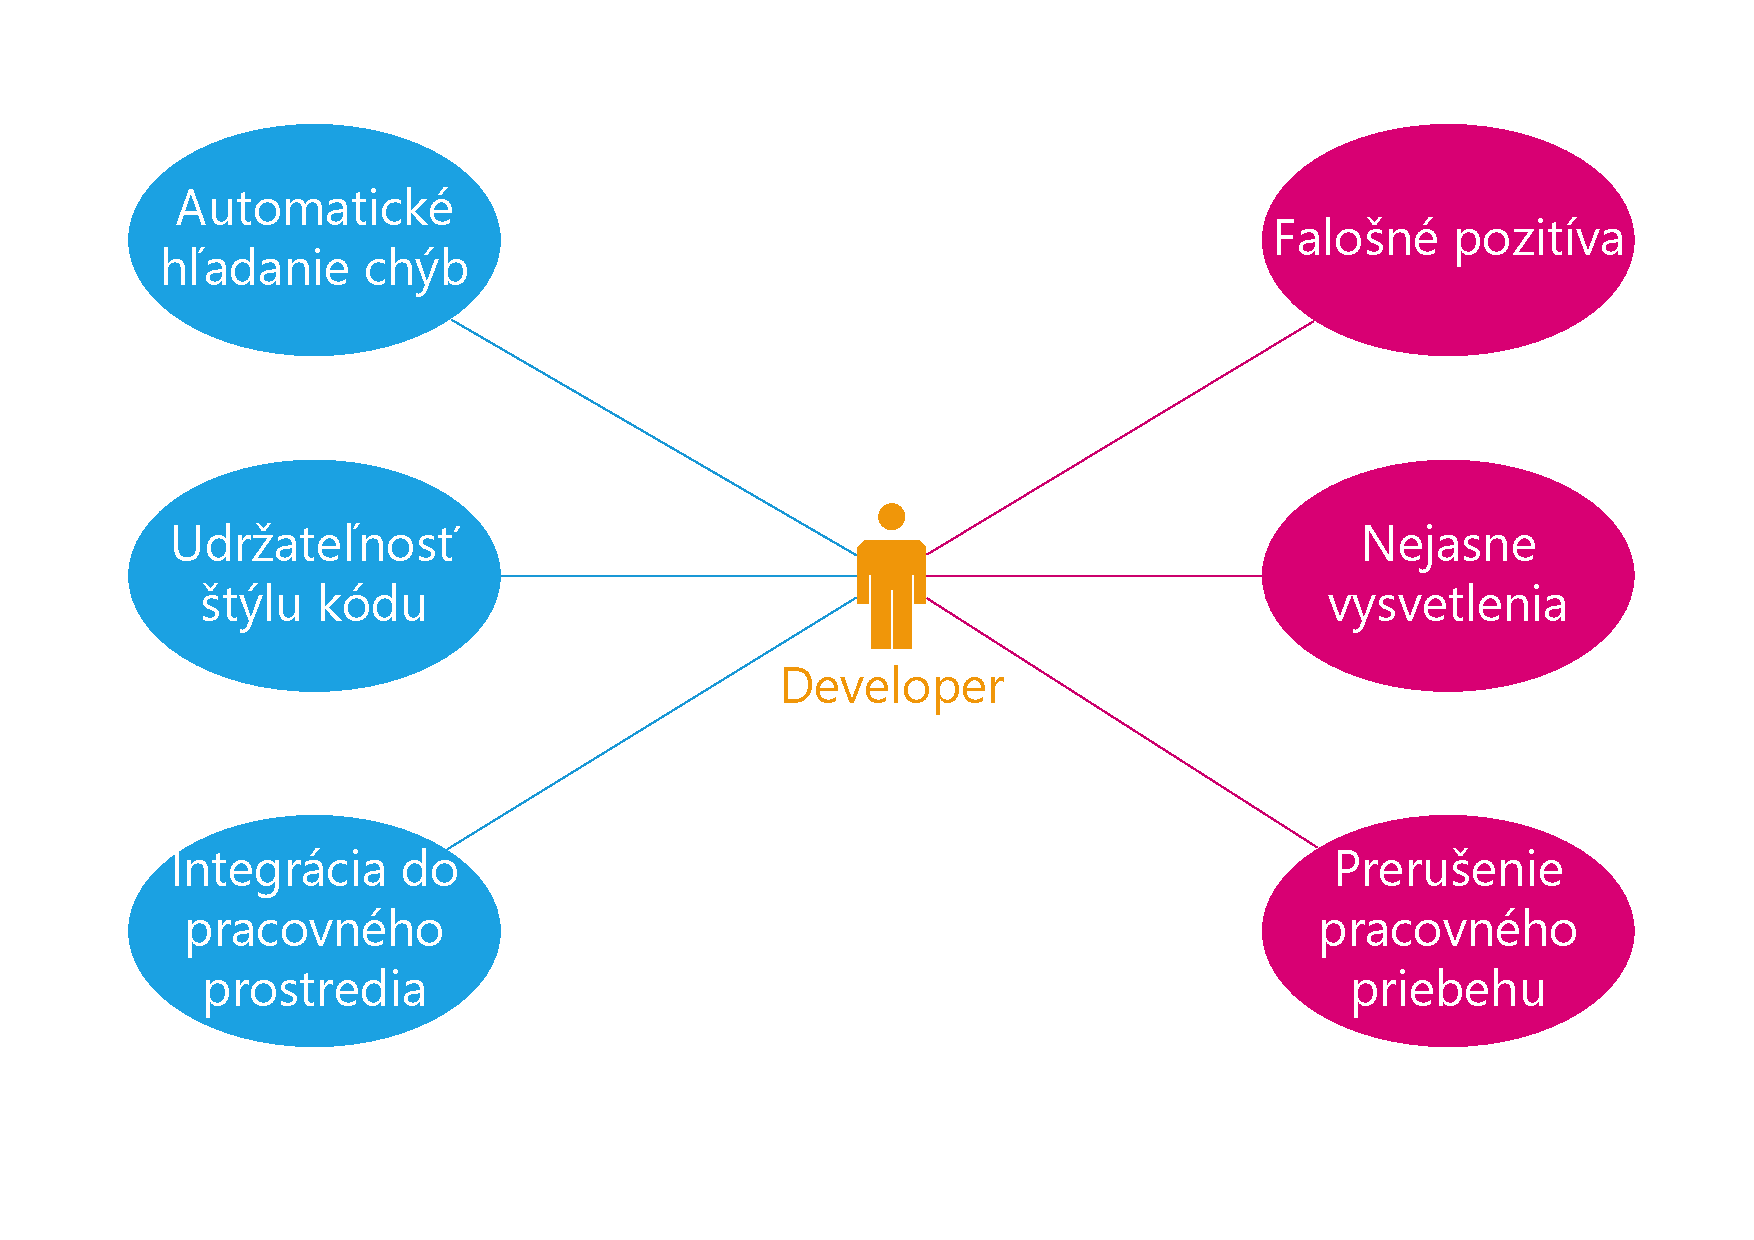
\includegraphics[scale=0.4]{pozitiva_negativa.pdf}}

\pagebreak
\bibliography{literatura}
\bibliographystyle{ieeetr}

\end{document}
